\chapter{Previous Designs and Implementations}\label{sec:previous-designs}

% TODO - add a note that all approaches are based on system model for synchronous risk propagation, and execute offline
Before working on ShareTrace, I did not have experience developing distributed algorithms. The approach proposed in \Cref{ch:risk-propagation} is my \emph{fifth} attempt\footnote{In completing this thesis, I have learned two important rules: define requirements clearly and recognize when those requirements are (not) satisfied. The time and effort needed for this thesis could have been significantly reduced had I adhered to these two simple rules.} at defining a performant implementation of risk propagation that satisfies the requirements of being decentralized and online. The prior four attempts offered valuable learnings that guided me toward the proposed approach. In fact, the approach defined in \Cref{sec:projected-subgraphs} is the topic of published work \cite{Tatton2022}. To document my efforts in developing this thesis, prior designs and implementations are provided in this appendix.

\section{Thinking Like a Vertex}\label{sec:giraph}

The first iteration of risk propagation \cite{Tatton2020} utilized Apache Giraph \cite{Giraph2020}, an open-source version of the iterative graph-processing library, Pregel \cite{Malewicz2010}, which is based on the bulk synchronous parallel model of distributed computing \cite{Valiant1990}. Giraph follows the \define{``think like a vertex'' paradigm} in which the algorithm is specified in terms of the local information available to a graph node \cite{McCune2015}.

% TODO - define Personal Data Accounts?
% TODO - Add Google/Apple citation
% TODO - is it ephemeral identifiers or EphID?
Risk propagation was implemented as defined in \cite{Ayday2020,Ayday2021}, using the factor graph representation of the contact network. However, because the Google/Apple API does not permit remotely persisting ephemeral identifiers, the implementation assumed that user geolocation data would be analyzed to generate the factor nodes in the factor graph (\Cref{sec:location-based}). \Cref{fig:aws-architecture} describes the high-level architecture. Callouts 1, 2, and 4 were implemented using a fan-out design pattern in which a \define{ventilator} Lambda function divides the work amongst \define{worker} Lambda functions.

\begin{figure}[htbp]
\centering
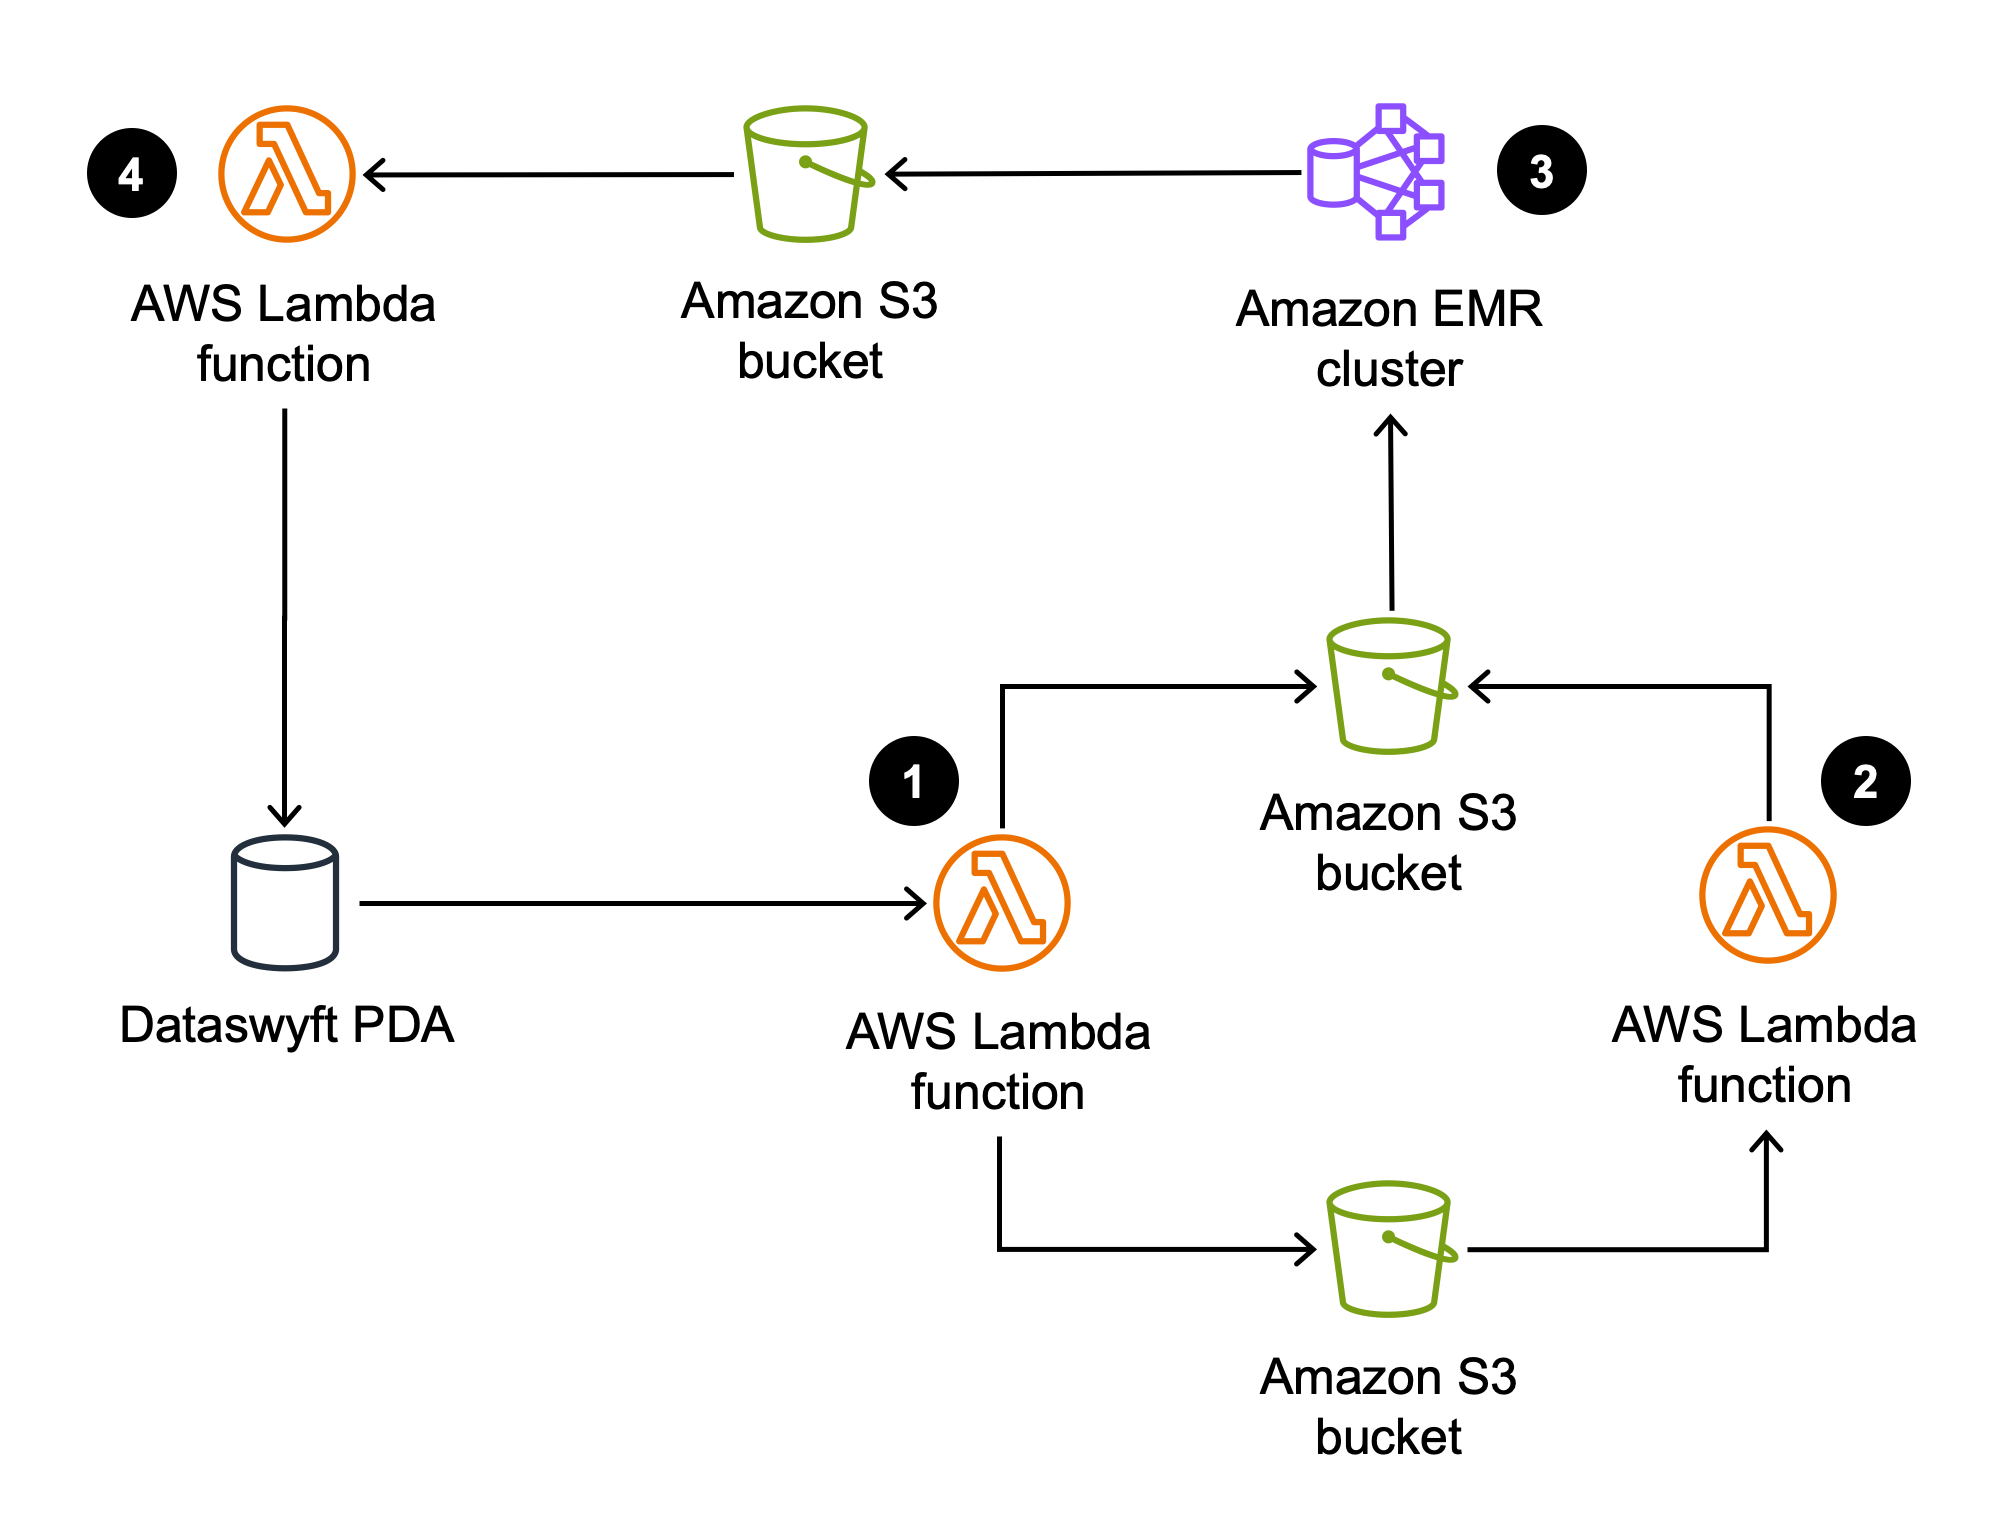
\includegraphics[width=\textwidth]{aws-architecture}
\caption[ShareTrace batch-processing architecture]{ShareTrace batch-processing architecture. (1) An AWS Lambda function retrieves the recent risk scores and location data from the Dataswyft Personal Data Accounts (PDAs) of ShareTrace users. Risk scores are formatted as Giraph nodes and stored in an Amazon Simple Storage Service (S3) bucket. Location data is stored in a separate S3 bucket. (2) A Lambda function performs a contact search over the location data and stores the contacts as Giraph edges in the same bucket that stores the Giraph nodes. (3) Amazon Elastic MapReduce (EMR) runs risk propagation as a Giraph job and stores the exposure scores in an S3 bucket. (4) A Lambda function stores the exposure score of each user in their respective PDA.}
\label{fig:aws-architecture}
\end{figure}

Several factors prompted me to search for an alternative implementation.

\begin{enumerate}
  \item \emph{Dependency management incompatibility}. A major cause for redesigning the implementation was the dependency version conflicts between Giraph and the other libraries. In spite of several attempts (e.g., using different library versions, using different versions of Giraph, and forcing specific transitive dependency versions) to resolve these conflicts, a lack of personal development experience and stalled progress prompted me pursue other approaches of implementation.
  \item \emph{Implementation complexity}. For a relatively straightforward data flow, the architecture in \Cref{fig:aws-architecture} corresponds to over 4,000 lines of source code. In retrospect, AWS Step Functions could have been used to orchestrate the workflow, including the fan-out design pattern, which would have simplified the Lambda function implementations. Regarding the implementation of risk propagation, one-mode projection onto variable nodes (first used in \Cref{sec:projected-subgraphs}) would have simplified the implementation since it avoids multiple node types, multiple message types, and enables the encapsulation of state and message-passing behavior.
  \item \emph{External data persistence}. One of the core tenets of Dataswyft is that the user fully controls the access to their data. However, as shown in \Cref{fig:aws-architecture}, user data is stored in S3 buckets. While it is possible to encrypt S3 objects at rest and enforce a short data retention policy, data persistence to any extent is suboptimal for \emph{privacy-preserving} digital contact tracing.
\end{enumerate}

\section{Subgraph Actors}\label{sec:subgraph-actors}

In an attempt to simplify the design in \Cref{sec:giraph}, I rewrote risk propagation using Ray, a Python library that ``aims to provide a universal API for distributed computing'' \cite{RayArchitecture}. While it claims to support actor-based programming, Ray only offers coarse-grained concurrency, with each actor being mapped to a machine processor. As with \Cref{sec:giraph}, I assumed the factor graph representation of the contact network. To achieve parallelism, the factor graph is partitioned amongst the actors such that each actor maintains a subset of variable nodes \emph{or} factor nodes. The graph topology is stored in shared memory so that all actors can efficiently access it. The lifetime of this design was brief for the following reasons.

\begin{enumerate}
\item \emph{Poor performance}. Communication between Ray actors requires message serialization. Moreover, partitioning the factor graph into subsets of factor and variable nodes results in maximal interprocess communication. Unsurprisingly, this choice of partitioning manifested in slow runtime performance.
\item \emph{Design complexity}. Not using a framework, like Giraph, meant that this implementation required more low-level code to implement actor functionality and message passing. Regardless of the performance, the overall design of this implementation was poorly organized and overthought.
\end{enumerate}

\section{Driver-Monitor-Worker Framework}\label{sec:mwd-framework}

Based on the poor runtime performance and complexity of the approach taken in \Cref{sec:subgraph-actors}, I speculated that centralizing the mutable aspects of risk propagation (i.e., the current value of each variable node) would improve both metrics. With this is mind, I designed the \define{monitor-worker-driver} (MWD) \define{framework}, which draws inspiration from the \define{tree of actors} design pattern \cite{RayTreeOfActors}. \Cref{fig:mwd-framework} describes the framework.

\begin{figure}[htbp]
\centering
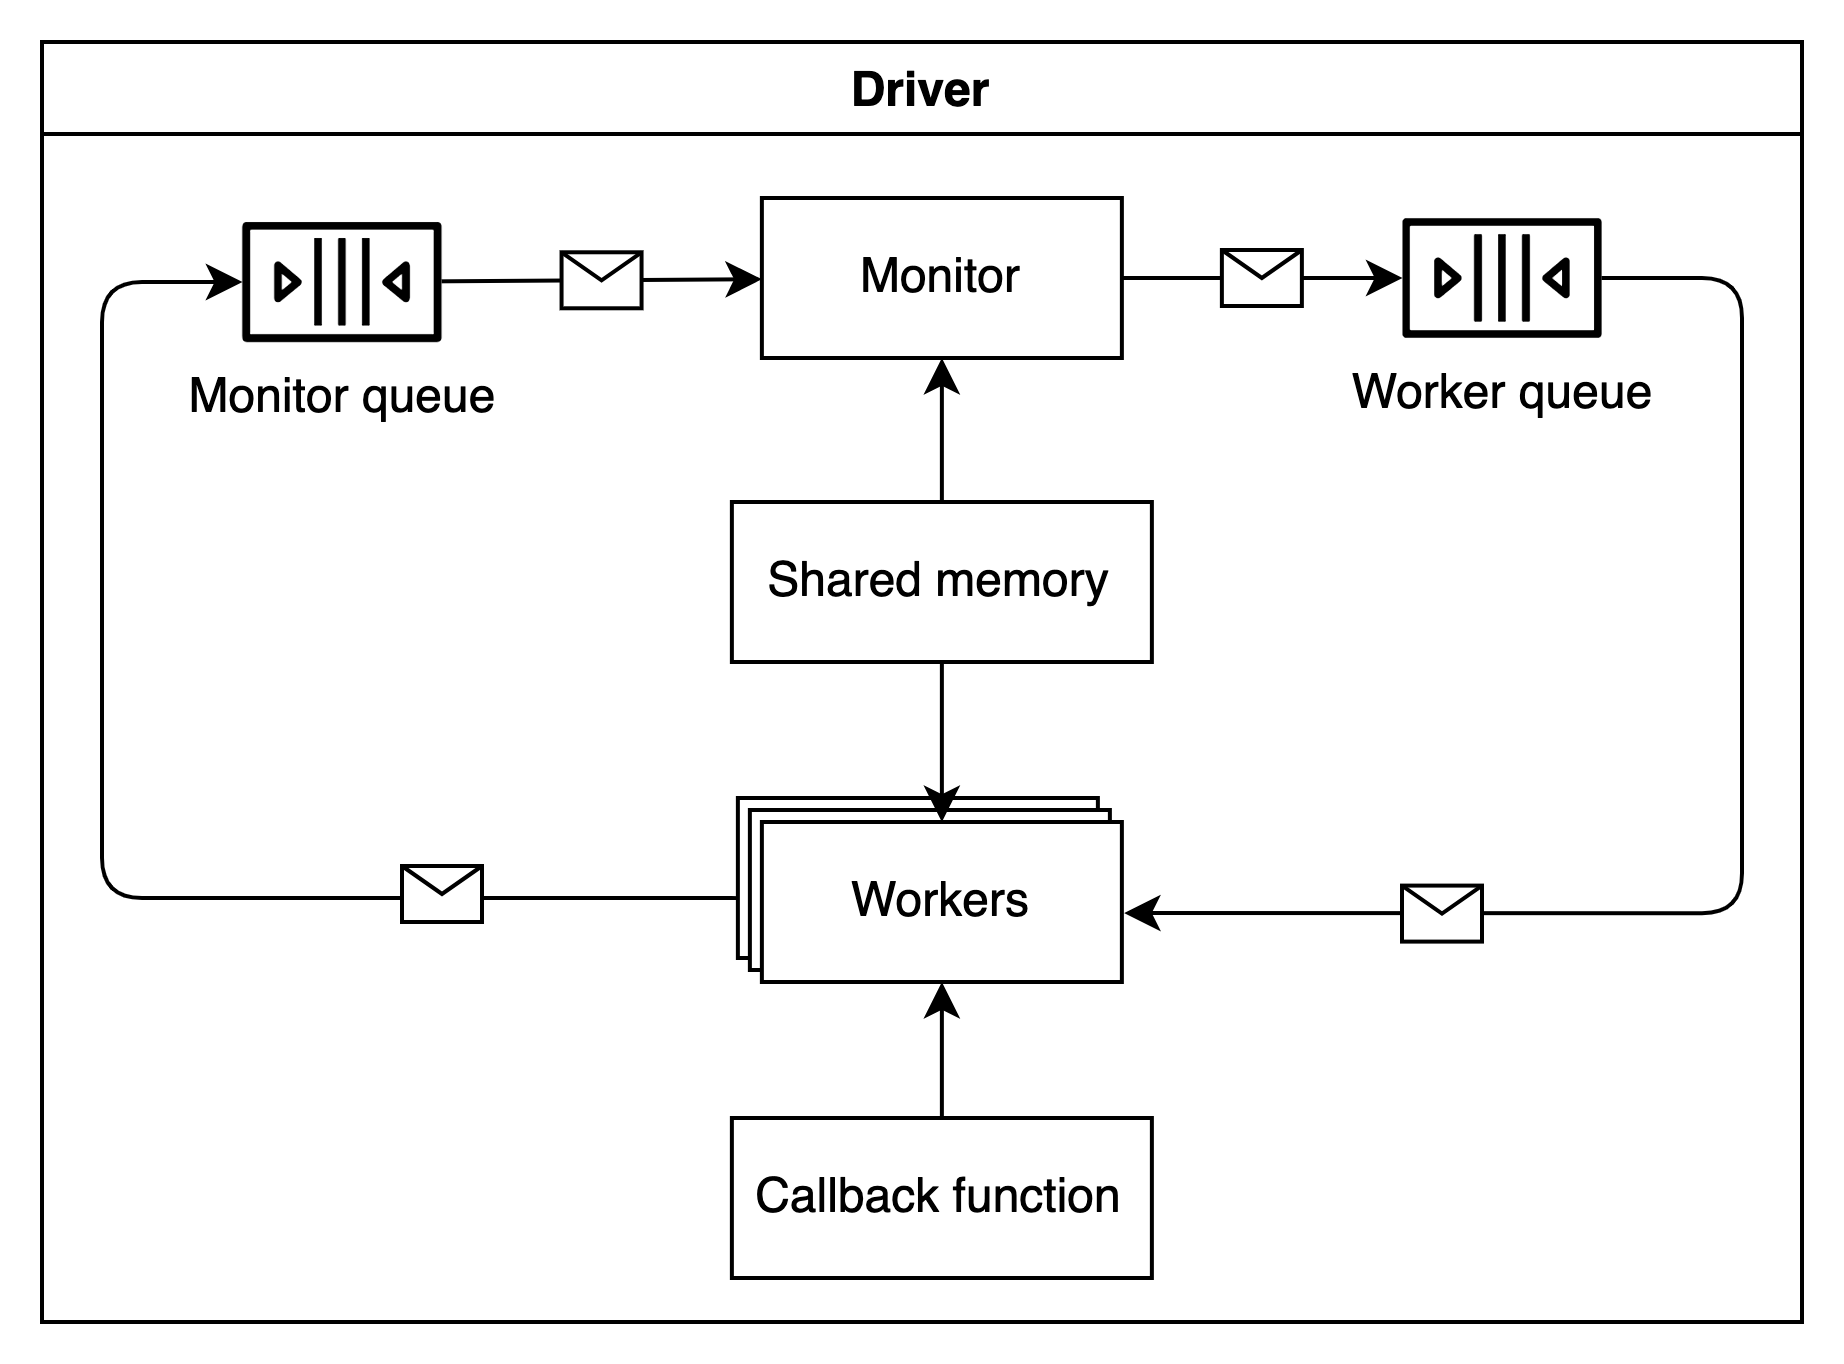
\includegraphics[width=\textwidth]{mwd-framework}
\caption[Monitor-worker-driver framework]{Monitor-worker-driver framework. The \define{monitor} encapsulates the mutable state of the program and decides which messages are processed by workers. A \define{worker} is a stateless entity that processes the messages that the monitor puts in the \define{worker queue}. Worker behavior is defined by a \define{callback function}, which typically depends on the message contents. The side effects of processing a message are recorded as new messages and put in the \define{monitor queue}. This cycle repeats until some termination condition is satisfied. Any immutable state of the program can be stored in \define{shared memory} for efficient access. The \define{driver} is the entry point into the program. It initializes the monitor and workers, and then waits for termination.}
\label{fig:mwd-framework}
\end{figure}

For risk propagation, the driver creates the factor graph from the set of risk scores $\vScores$ and contacts $\vContacts$, stores the factor graph in shared memory, sets the initial state of the monitor to be the maximum risk score of each user, and puts all risk scores in the monitor queue. During message passing, the monitor maintains the maximum risk score (i.e., exposure score) for each variable node.

The MWD framework was the first approach that utilized the send coefficient to ensure the convergence and termination of message passing. However, because the MWD-based implementation assumed the factor graph representation of the contact network, the send coefficient was applied to both variable and factor messages.

Compared to the approach in \Cref{sec:subgraph-actors}, this implementation provides a cleaner design and less communication overhead. However, what prompted me to consider (yet another) an alternative implementation was its scalability. Because the monitor processes messages serially, it is a bottleneck for algorithms in which the workers perform fine-grained tasks. Indeed, the Ray documentation notes that the parallelization of small tasks is an anti-pattern because the interprocess communication cost exceeds the benefit of multiprocessing \cite{RayFineGrainedTasks}. Unfortunately, the computation performed by factor nodes and variable nodes is too fine-grained, so the scalability of the MWD framework was demonstrably poor.

\section{Projected Subgraph Actors}\label{sec:projected-subgraphs}

\section{Location-Based Contact Tracing}\label{sec:location-based}
	\begin{itemize}
	\item Motivation: Google/Apple API prevents exporting Bluetooth EphIDs
	\item Other location-based contact tracing approaches
	\end{itemize}
\subsection{System Model}
The system model is very similar to previous work \cite{Ayday2020, Ayday2021} and designs. The only difference is that user geolocation data is collected instead of Bluetooth ephemeral identifiers. \Cref{fig:location-based} shows the modified dataflow\footnote{See \cref{foot:dataflow} (p. \labelcpageref{foot:dataflow}) for the definition of a dataflow diagram.}.
	\begin{figure}[ht!]
		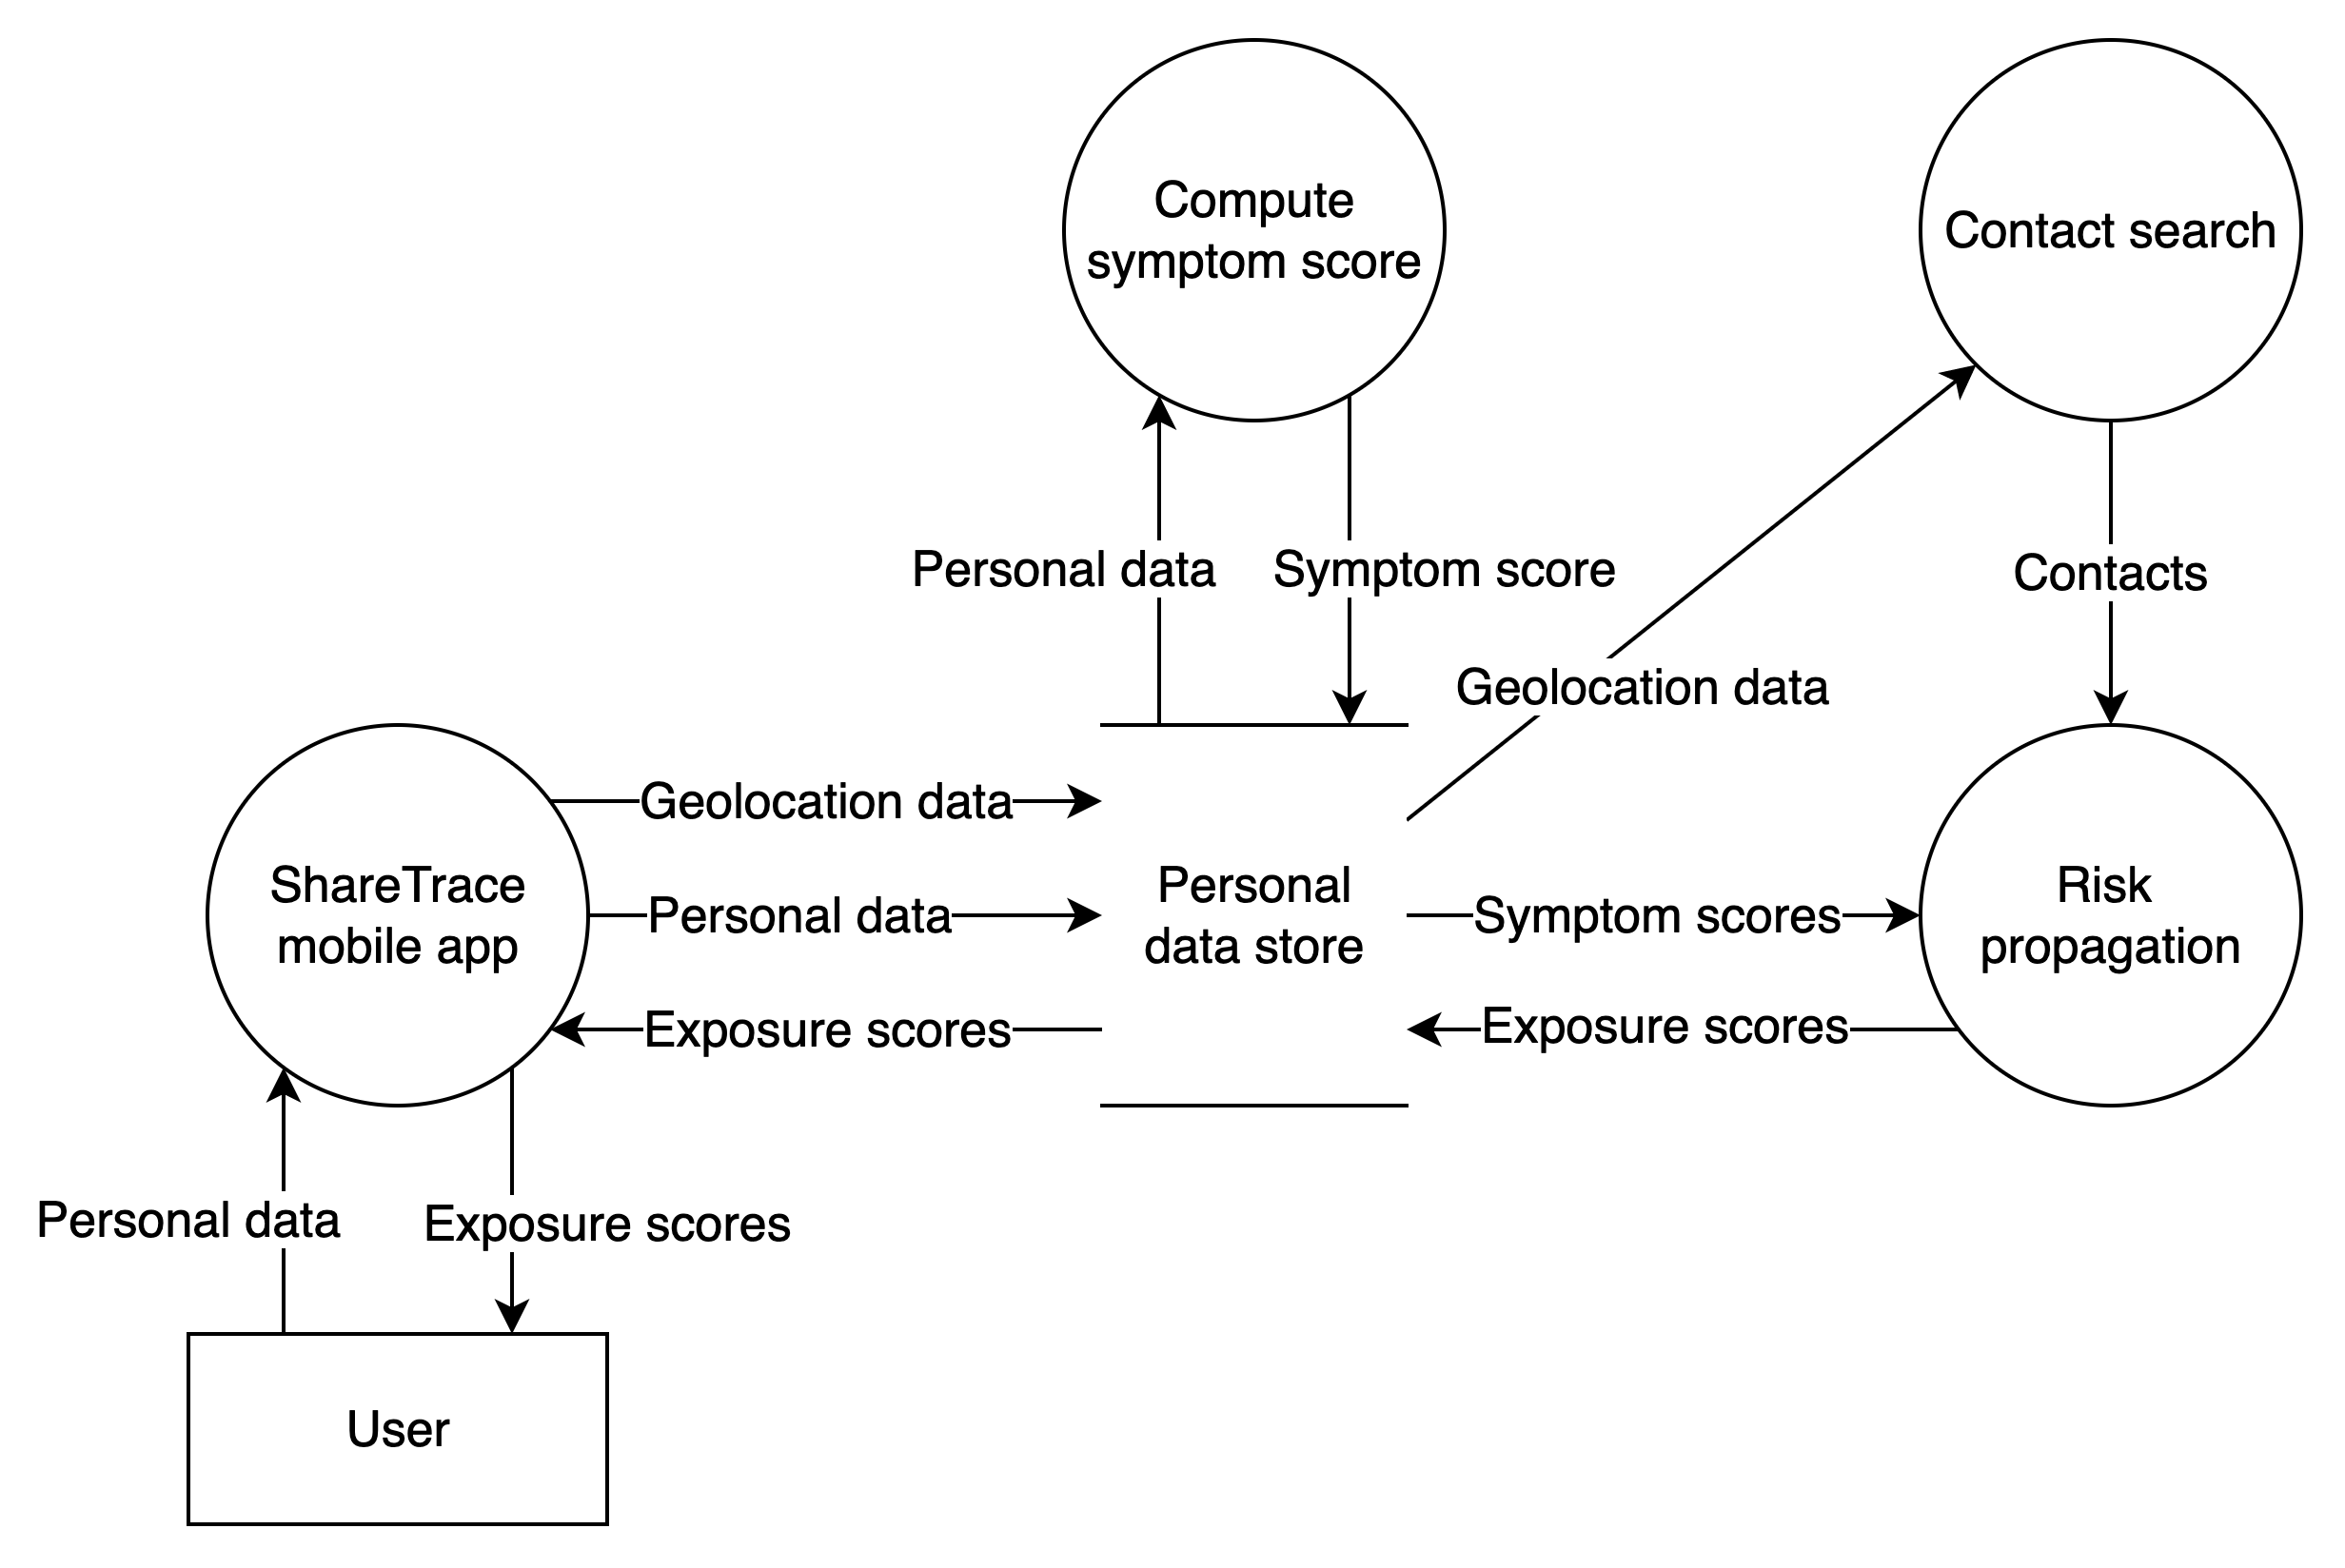
\includegraphics[width=\textwidth]{location-dataflow}
		\caption[Geolocation-based ShareTrace dataflow]{Location-based ShareTrace dataflow. This requires that risk propagation is executed in a centralized setting since all user geolocation data is needed to construct the contact network.}
		\label{fig:location-based}
	\end{figure}
\define{Geohashing} is a public-domain encoding system that maps \define{geographic coordinates} (i.e., latitude-longitude ordered pairs \cite[p. 5]{Sickle2004}) to alphanumeric strings called \define{geohashes}, where the length of a geohash is correlated with its geospatial precision \cite{Morton1966}. To offer some basic privacy, a user's precise geolocation history is obfuscated on-device by encoding geographic coordinates as geohashes with 8-character precision which corresponds to a region of $730\mathrm{m}^2$.

\subsection{Contact Search}

\newcommand{\histories}{\mathcal{H}}
\newcommand{\locations}{\mathbb{L}}
\newcommand{\locset}{\mathcal{L}}
\newcommand{\latitude}{\phi}
\newcommand{\longitude}{\lambda}
\newcommand{\users}{\mathcal{U}}
\newcommand{\sindex}{\mathcal{I}}
\newcommand{\query}{\mathcal{N}}
\newcommand{\qelement}{q}
\newcommand{\hone}{G}
\newcommand{\htwo}{H}
\newcommand{\neighbors}{N}

A \define{contact} follows the definition of \eqref{eq:contact-seq}, where the contact time $\tsym$ indicates the most recent time at which two users were proximal for a contiguous duration of at least $\delta \in \preals$. Each user has a \define{geolocation history}
	\begin{equation*}
		\htwo = \left[(\tsym_i, \ell_i) \mid ~\forall i \in \ints_{[1, \attr{\htwo}{length}]} (\tsym_i < \tsym_{i + 1}) \right],
	\end{equation*}
a temporally ordered sequence of timestamped geolocations. It is assumed that
	\begin{enumerate}
		\item geolocation histories are not recorded on a fixed schedule, and \label{assume:sched}
		\item a user remains at a geolocation until the next geolocation is recorded. \label{assume:static}
	\end{enumerate}
By assumption \ref{assume:sched}, any two geolocation histories can be ``out of alignment'' such that they are of different length with interleaving timestamps. Geolocation histories $\hone, \htwo$ can be \define{aligned} by \define{padding} such that
	\begin{equation*}
		n = \attr{\hone}{length} = \attr{\htwo}{length},
	\end{equation*}
and \define{temporally interpolating} such that
	\begin{equation*}
		\forall i \in \ints_{[1, n]}(\timeAttr{\hone[i]} = \timeAttr{\htwo[i]}).
	\end{equation*}
By assumption \ref{assume:static}, it is most appropriate to use \define{previous interpolation}: given timestamped geolocations $(\tsym_i, \ell_i), (\tsym_j, \ell_j)$ such that $\tsym_i < \tsym_j$, all intermediate geolocations are defined as $(\tsym_k, \ell_i)$ for all $\tsym_k \in [\tsym_i, \tsym_j)$. In practice, time is a discrete variable that is recorded with fixed precision (e.g., seconds). Let $T \in \pints$ be the \define{time period} between two consecutive timestamps $\tsym_i, \tsym_{i + 1}$ such that $\tsym_{i + 1} = \tsym_i + T$. Then previous interpolation between timestamps $\tsym_i, \tsym_j$ such that $\tsym_j > \tsym_i$ results in $T \cdot (\tsym_j - \tsym_i - 1)$ intermediate geolocations.

Finding the most recent contact between two users from their aligned geolocation histories is similar to finding the last $k$-length common substring between two strings, where each symbol represents a timestamped geolocation. The difference lies in how the start and end of the contact time interval is defined. By assumption \ref{assume:static}, the start (end) of a contact time interval is defined as the earlier (ref. later) timestamp of the two first (ref. last) timestamped geolocations in the sequence where the two histories differ. \Cref{fig:contact-search} provides a visual example.
	\begin{figure}[ht!]
	    \centering
	    \begin{tikzpicture}[scale=2]
	        \draw[latex-latex] (-3,0) -- (3,0);
	        \draw[latex-latex] (-3, 1) -- (3,1);
	        \draw (-2,0) -- (-2,1);
	        \draw (-1.5,0) -- (-1.5,1);
	        \draw (0.5,0) -- (0.5,1);
	        \draw (2,0) -- (2,1);
	        \draw (-1.75, 0.5) node {$A$};
	        \draw (1.25, 0.5) node {$B$};

	        \path [draw=black, fill=black] (-2,0) circle (1pt);
	        \path [draw=black, fill=black] (0,0) circle (1pt);
	        \path [draw=black, fill=black] (2,0) circle (1pt);
	        \path [draw=black, fill=black] (-2.5,1) circle (1pt);
	        \path [draw=black, fill=black] (-1.5,1) circle (1pt);
	        \path [draw=black, fill=black] (0.5,1) circle (1pt);
	        \path [draw=black, fill=black] (2.5,1) circle (1pt);

	        \node[below=2pt of {(-2,0)}] {$\ell_1$};
	        \node[below=2pt of {(0,0)}] {$\ell_3$};
	        \node[below=2pt of {(2,0)}] {$\ell_2$};
	        \node[above=2pt of {(-2.5,1)}] {$\ell_1$};
	        \node[above=2pt of {(-1.5,1)}] {$\ell_2$};
	        \node[above=2pt of {(0.5,1)}] {$\ell_3$};
	        \node[above=2pt of {(2.5,1)}] {$\ell_1$};
	    \end{tikzpicture}
	    \caption[Contact search with two geolocation histories]{Contact search with two geolocation histories. Each line denotes time, increasing from left to right. A point $\ell_i$ is a geolocation and occurs relative in time with respect to the placement of other points. Region $B$ defines the contact interval as it is of sufficient duration and occurs after $A$.}
	    \label{fig:contact-search}
	    \end{figure}

\subsubsection{Naive Contact Search}\label{sec:naive-contact-search}
A naive approach to finding all contacts amongst a set of geolocation histories $\histories$ is to compare all unordered pairs. For a given pair of aligned geolocation histories, the idea is to maintain a pointer to the previous and current index in each history, advancing the pair of pointers whose geolocation occurs later in time. Once a common geolocation is found, all pointers are advanced together until the geolocations differ. If the sequence is $\delta$-contiguous, where a sequence of timestamped geolocations $S$ is \define{$\delta$-contiguous} if $\attr{S}{length} \geq \delta$ and
	\begin{equation*}
		\forall i \in \ints_{[1, \attr{S}{length}]}(\timeAttr{S[i + 1]} = \timeAttr{S[i]} + T),
	\end{equation*}
then it is recorded. The latest such sequence is used to define the contact between the two users. Because only the most recent time of contact is of interest, the procedure can be improved by iterating in reverse and then terminating once a sequence is found. Regardless, this approach takes $\Theta(n^2)$ time, where $n = \card{\histories}$, because all $\frac{n(n - 1)}{2}$ unique pairs must be considered.

The \Call{Naive-Contact-Search}{} operation implements the above procedure. The operation \Call{Most-Recent-Contact}{} considers geolocations\footnote{The symbol ``$\locations$'' denotes the space of all geolocations.} $\ell_i, \ell_j \in \locations$ \define{$\epsilon$-proximal} (i.e., approximately equal) if $d(\ell_i, \ell_j) \leq \epsilon$, according to some \define{metric} $d: \locations \times \locations \rightarrow \nnreals$ \cite[p. 118]{Kelley1975} and distance $\epsilon \in \nnreals$. Because geolocations are encoded as geohashes, they must be decoded into geographic coordinates to perform this proximity calculation. Moreover, because geohashing discretizes the coordinate system into a grid of geographic regions, the number of possible geolocations is finite. Thus, the operation returns a $\delta$-contiguous, $\epsilon$-proximal contact $c$ if such a contact exists between the geolocation histories $\hone, \htwo \in \histories$. The \Call{Align-Histories}{} operation pads each geolocation history such that the padded values (e.g., $\pm \infty$) do not result in false contact between users.
	\begin{algorithm}[ht!]
	\begin{algorithmic}[1]
		\Title{Naive-Contact-Search}{\histories}
		\State $\contacts \assign \emptyset$
		\ForEach{$(\hone, \htwo) \in \Call{Unique-Pairs}{\histories}$}
			\State $(\hone, \htwo) \assign \Call{Align-Histories}{\hone, \htwo}$
			\State $\var{c} \assign \Call{Most-Recent-Contact}{\hone, \htwo, \epsilon, \delta}$
			\If{$\var{c} \notequals \nil$}
				\State $\contacts \assign \contacts \cup \{c\}$
			\EndIf
		\EndFor
		\State \Return $\contacts$
	\end{algorithmic}
	\end{algorithm}

\subsubsection{Indexed Contact Search}
While the \textbf{for} loop in \Call{Naive-Contact-Search}{} is \define{embarrassingly parallel} \cite[p. 14]{Herlihy2012}, the naive approach is neither scalable nor efficient. It can be improved by observing that it is necessary, but not sufficient, that a pair of $\epsilon$-proximal geolocations exists between two geolocation histories for a contact to exist. Therefore, the geolocation histories $\histories$ can be indexed into a spatial data structure $\sindex$ \cite{Mokbel2003, Dinh2010, Mahmood2019} and then only consider the geolocation-history pairs that share at least one $\epsilon$-proximal geolocation pair. This approach is described by the \Call{Indexed-Contact-Search}{} operation.

Line \ref{step:query} executes a fixed-radius near-neighbors search (FR-NNS) \cite{Bentley1975, Brin1995} for each geolocation in the spatial index $\sindex$. Formally, given a set of geolocations $\locset \subseteq \locations$, a metric $d$, and a distance $\epsilon$, the \define{fixed-radius near-neighbors} of a geolocation $\ell \in \locset$ is defined as the subset of $\epsilon$-proximal geolocations \cite{Brin1995},
	\begin{equation*}
		\query(\ell) = \{\ell' \in \locset \mid d(\ell, \ell') \leq \epsilon\}
	\end{equation*}

Note that the set of neighbors $\query(i)$ of user $i$ corresponds to the geolocations that are $\epsilon$-proximal to \emph{any} of the geolocations in their geolocation history $\htwo_i$,
	\begin{equation*}
		\query(i) = \bigcup_{\ell \in \htwo_i} \query(\ell).
	\end{equation*}
On line \ref{step:to-users}, the operation \Call{Unique-Users}{} maps these near-neighbors back to the associated users, removing any duplicates that may arise from mapping multiple geolocations to the same user. Finally, line \ref{step:subset} maps the set of users $\users$ back to their geolocation histories and runs \Call{Naive-Contact-Search}{} on the resultant subset.
	\begin{algorithm}[ht!]
	\begin{algorithmic}[1]
		\Title{Indexed-Contact-Search}{\histories}
		\State $\sindex \assign \Call{Spatially-Index}{\histories}$
		\State $\query \assign \Call{Fixed-Radius-Near-Neighbors}{\sindex, \epsilon}$ \label{step:query}
		\State $\users \assign \Call{Unique-Users}{\query, \histories}$ \label{step:to-users}
		\State \Return \Call{Naive-Contact-Search}{$\{\htwo_i \in \histories \mid i \in \users\}$} \label{step:subset}
	\end{algorithmic}
	\end{algorithm}

To carry out FR-NNS, one approach is to use a \define{ball tree}, a complete binary tree that associates with each node a hypersphere that contains a subset of the data \cite{Omohundro1989, Neeraj2008, Kibriya2007}. Any metric can be used to perform FR-NNS on a ball tree. However, because geolocation is represented as geographic coordinates, metrics that assume a Cartesian coordinate system may be unsuitable. One of the simplest geometric models of the Earth is that of a sphere. Given two geographic coordinates, the problem of finding the length of the geodesic\footnote{The \define{geodesic} is the shortest segment between two points on an ellipsoid \cite[p. 204]{Lu2014}.} between them is known as the \define{inverse geodetic problem} \cite{Sjoberg2012}. Assuming a spherical Earth, the solution to the inverse problem is to find the length of the segment that joins the two points on a great circle\footnote{The \define{great circle} is the cross-section of a sphere that contains its center \cite[p. 165]{Lu2014}}.

Let $\theta = \frac{d}{r}$ be the \define{central angle}, where $d \in \nnreals$ is the distance between the two points along the great circle of a sphere with radius $r \in \preals$ (see \Cref{fig:central-angle}).
	\def\myrad{2.25cm}% radius of the circle
	\def\myang{60}% angle for the arc
	\begin{figure}[ht!]
	\centering
	\begin{tikzpicture}
	% the origin
		\coordinate (O) at (0,0);
		% the circle and the dot at the origin
		\draw (O) node[circle,inner sep=1.5pt,fill] {} circle [radius=\myrad];
		% the ``\theta'' arc
		\draw
		  (\myrad,0) coordinate (xcoord) --
		  node[midway,below] {$r$} (O) --
		  (\myang:\myrad) coordinate (slcoord)
		  pic [draw,angle radius=1cm,"$\theta$"] {angle = xcoord--O--slcoord};
		% the outer ``s'' arc
		\draw[|-|]
		  (\myrad+10pt,0)
		  arc[start angle=0,end angle=\myang,radius=\myrad+10pt]
		  node[midway,fill=white] {$d$};
	\end{tikzpicture}
	\caption[Central angle of a great circle]{Central angle of a great circle.}
	\label{fig:central-angle}
	\end{figure}
The \define{haversine}, or the half ``versed'' (i.e., reversed) sine, of a central angle $\theta$ is defined as
	\begin{equation}
		\hav \theta = \frac{\vers \theta}{2}  = \frac{1 - \cos \theta}{2}= \sin^2 \frac{\theta}{2}. \label{eq:hav}
	\end{equation}
The great-circle distance $d$ between two points can be found by inversing \labelcref{eq:hav} and solving,
	\begin{equation*}
		d(\ell_i, \ell_j) = 2 \cdot \arcsin \sqrt{\sin^2 \frac{\latitude_i - \latitude_j}{2} + \cos \latitude_i \cdot \cos\latitude_j \cdot \sin^2 \frac{\longitude_i - \longitude_j}{2}},
	\end{equation*}
where $\ell_i = (\latitude_i, \longitude_i)$ is a latitude-longitude coordinate in radians \cite[pp. 157--162]{Brummelen2013}.

The choice of the great-circle distance was primarily driven by its readily available usage in the scikit-learn \cite{sklearn2013} implementation of a ball tree. If such an approach for discovering contacts were to be used in practice, more advanced \define{geodetic datum} \cite[pp. 71--130]{Lu2014} could be used to provide better geospatial accuracy. Moreover, by projecting geodetic coordinates onto the plane, metrics that assume a Cartesian coordinate system could be used instead \cite[pp. 265--326]{Lu2014}.

The running time of \Call{Spatially-Index}{} is $\Theta\left(\card{\histories} \cdot \log\card{\histories}\right)$ \cite{Omohundro1989}. Assuming the ball tree is balanced\footnote{The ball-tree implementation provided by scikit-learn \cite{sklearn2013} ensures the tree is balanced.}, the running time of \Call{Fixed-Radius-Near-Neighbors}{} to find the $\epsilon$-proximal neighbors of all geolocations in the spatial index $\sindex$ is $\Theta(k \card{\sindex} \cdot \log\card{\sindex})$ , where $k$ is the dimensionality of a tree element (i.e., $k = 2$ for geographic coordinates). The running time of \Call{Unique-Users}{} is $\Theta(\card{\query})$. While the running time of \Call{Naive-Contact-Search}{} is $\Theta\left(\card{\users}^2\right)$, it is likely that $\card{\users} << \card{\histories}$. Regardless of the input,
	\begin{equation*}
		\card{\histories} \geq \card{\sindex} \geq \card{\users}
	\end{equation*}
since $\card{\histories} = \card{\sindex}$ only if all geolocations in $\histories$ are distinct, and $\card{\sindex} = \card{\users}$ only if each user has exactly one geolocation that is distinct from all other users. Dependent upon the input, however, is $\card{\query}$. In the worst case, $\card{\query} \in O\left(\card{\sindex}^2\right)$ if each geolocation is $\epsilon$-proximal to all other geolocations. This implies that the overall worst-case running time of \Call{Indexed-Contact-Search}{} is $O(\card{\histories}^2)$. In practice, the running time depends on the geohash precision as well as the geospatial density and mobility behavior of the user population.

\subsection{Closing Remarks}

% Common short-comings and learnings of all previous approaches
% Issues with location-based contact tracing:
%   - Privacy
%   - GPS fine-grained accuracy and power consumption
%   - Downstream accuracy of risk propagation
%   - Scalability